% --------------------------------------------------------------
% This is all preamble stuff that you don't have to worry about.
% Head down to where it says "Start here"
% --------------------------------------------------------------

\documentclass[12pt]{article}

\usepackage[margin=1in]{geometry} 
\usepackage{amsmath,amsthm,amssymb}
\usepackage{color}
\usepackage{fancyhdr}
\usepackage{lastpage}
\usepackage{graphicx}
\usepackage{subcaption}
\usepackage{url}
\usepackage{pdfpages}

\pagestyle{fancy}
\fancyhf{}
\fancyhead[L]{ID: 6110}
%\fancyhead[C]{\thepage}
%\fancyhead[R]{Module 5 Homework}
\fancyhead[C]{Project 4}
\fancyhead[R]{Prof. Hicken, MANE 4280}

\rfoot{Page \thepage \hspace{1pt} of \pageref{LastPage}}

\newcommand{\N}{\mathbb{N}}
\newcommand{\Z}{\mathbb{Z}}

\newenvironment{theorem}[2][Theorem]{\begin{trivlist}
		\item[\hskip \labelsep {\bfseries #1}\hskip \labelsep {\bfseries #2.}]}{\end{trivlist}}
\newenvironment{lemma}[2][Lemma]{\begin{trivlist}
		\item[\hskip \labelsep {\bfseries #1}\hskip \labelsep {\bfseries #2.}]}{\end{trivlist}}
\newenvironment{exercise}[2][Exercise]{\begin{trivlist}
		\item[\hskip \labelsep {\bfseries #1}\hskip \labelsep {\bfseries #2.}]}{\end{trivlist}}
\newenvironment{problem}[2][Problem]{\begin{trivlist}
		\item[\hskip \labelsep {\bfseries #1}\hskip \labelsep {\bfseries #2.}]}{\end{trivlist}}
\newenvironment{question}[2][Question]{\begin{trivlist}
		\item[\hskip \labelsep {\bfseries #1}\hskip \labelsep {\bfseries #2.}]}{\end{trivlist}}
\newenvironment{corollary}[2][Corollary]{\begin{trivlist}
		\item[\hskip \labelsep {\bfseries #1}\hskip \labelsep {\bfseries #2.}]}{\end{trivlist}}

\newenvironment{solution}{\begin{proof}[Solution]}{\end{proof}}
\usepackage{multicol}
\newcommand{\mysize}{0.5}
\usepackage{subcaption}
\usepackage{float}
\usepackage{listings}
\usepackage{color} %red, green, blue, yellow, cyan, magenta, black, white
\definecolor{mygreen}{RGB}{28,172,0} % color values Red, Green, Blue
\definecolor{mylilas}{RGB}{170,55,241}


\begin{document}
	
	% --------------------------------------------------------------
	%                         Start here
	% --------------------------------------------------------------
	
	\title{Project 4: Uncertain Loading of a UAV Spar}
	\author{ID: 6110\\ %replace with your name
		 MANE 4280, Design Optimization}
	
	\maketitle
	\tableofcontents
	\thispagestyle{empty}
	\newpage
	\setcounter{page}{1}
	\section{Executive Summary}


	A spar is a type of support found in the wing of an aeroplane. Used as early as the Wright brother's days, spars are used in plane wings today to provide structural support, and to transport the forces acting on the wings to the rest of the plane. 
	
	\begin{figure}[h!]
		\centering
		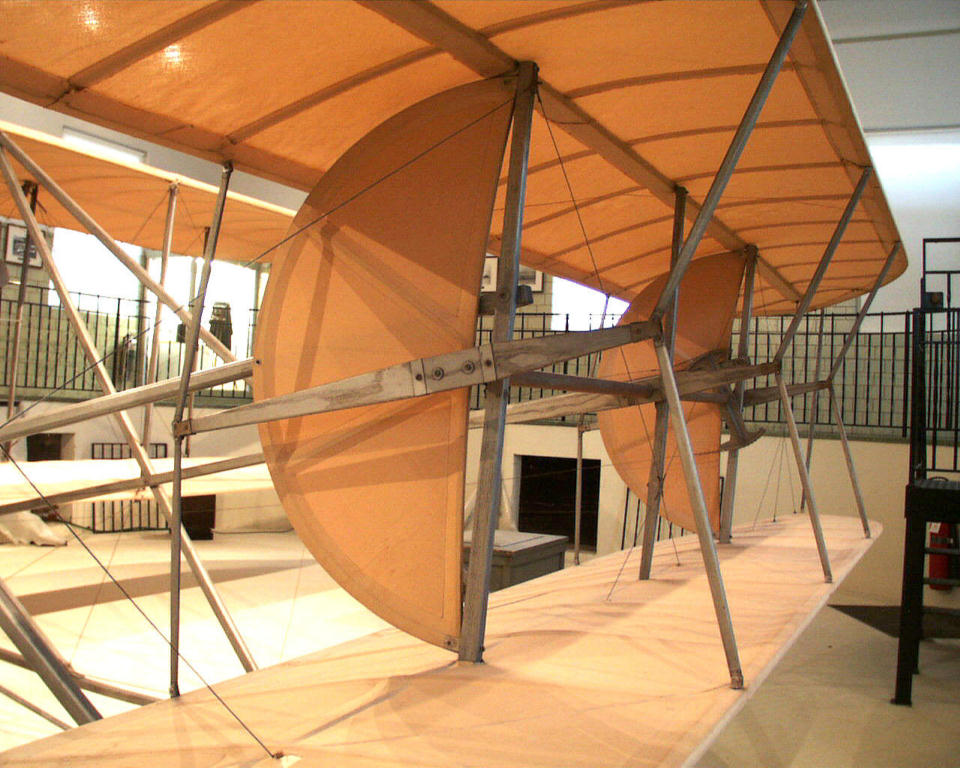
\includegraphics[width=0.5\linewidth]{sparFlyer}
		\caption{Spars and ribs are visible in the aerofoils of the Wright brother's Flyer\cite{original1905wrightflyeriii}.}
		\label{fig:sparflyer}
	\end{figure}
	
	
	A spar similar to the type explored in this project is seen in figure \ref{fig:spardiagram} %\ref{fig:telescopicwing}\cite{afa}
	
	\begin{figure}[h!]
	\centering
	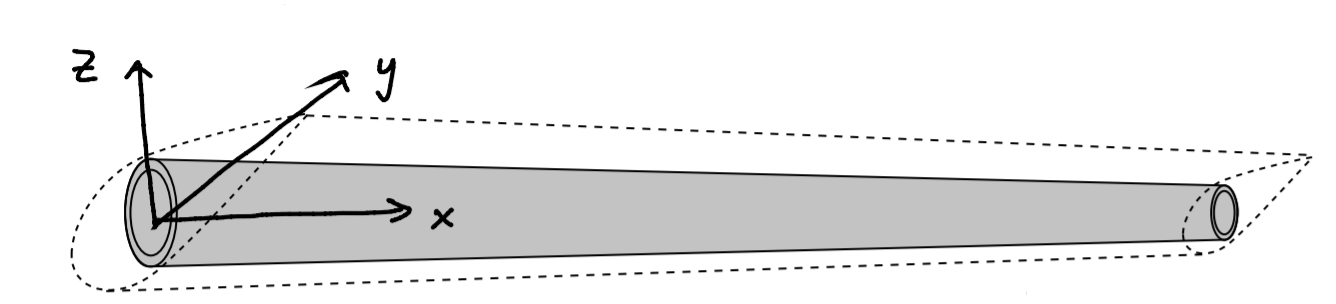
\includegraphics[width=0.7\linewidth]{sparDiagram}
	\caption{Diagram of spar with axis \cite{Hicken18}.}
	\label{fig:spardiagram}
\end{figure}



	The goal of this project is to develop an optimal design for a spar that will minimize the mass under uncertain loading subject to a given set of constraints. This report will explain the analysis methods and their limitations, discuss how the geometry was parameterized, investigate the optimization methods and their results.
	
	

	
	
	\section{Analysis Methods}	
	Before the analysis begins the details of the spar should be listed. It has a length of 7.5 meters. It's density is 1,600 $\frac{kg}{m^3}$\cite{Hicken18Proj}. A diagram of the spar is seen in figure \ref{fig:spardiagram}. The minimum radius of the spar is one centimeter and the maximum radius is five centimeters. The thickness must be greater than 2.5 mm. The bending of the spar is modeled by Euler-Bernoulli Beam Theory using the following equations\cite{Hicken18}.
	
	\begin{equation}
	\frac{d^2}{dx^2}\left(EI_{yy}\frac{d^2 w}{dx^2}\right)=q,  \forall x\in[0,L]
	\end{equation}
	
	Where 
	\begin{align}
	w& \text{ is the vertical displacement in the z direction (m)}\nonumber\\
	q(x)& \text{ is the applied load (N/m)}\nonumber\\
	E& \text{ is the elastic, or Young’s, modulus (Pa)}\nonumber\\
	I_{yy}& \text{ is the second-moment of area with respect to the y axis }\text{(m)}^2\nonumber
	\end{align}
	\begin{equation}
	I_{yy}=\int \int z^2 dz dy
	\end{equation}
	The spar is treated like a cantilever beam with the following boundary conditions:
	\begin{align}
	w(x=0)=0,&\text{   } \frac{d^2w}{dx^2}(x=L)=0\\
	\frac{dw}{dx}(x=0)=0,&\text{   }\frac{d^3w}{dx^3}(x=L)=0
	\end{align}
	This is to say that there is no vertical or angular displacement at the root and no stress at the tip. Once the vertical displacement is known, the stress may be solved by
	\begin{equation}
\sigma_{xx} (x)=-z_{max}E\frac{d^2w}{dx^2}
	\end{equation}
	
	The beam is discretized by the finite-element method. The finite-element equations come from the minimization of the potential energy. The solution is represented using Hermite-cubic shape functions. It is assumed that the spar does not experience any thermal effects due to the warping or the atmosphere's temperature. 
	
	The load on the spar is described by 
	
	\begin{equation}
	f ( x , \xi ) = f _ { \mathrm { nom } } ( x ) + \delta _ { f } ( x , \xi )
	\end{equation}
	Where 
	\begin{equation}
	f _ { \mathrm { nom } } ( x ) = \frac { 2.5 W } { L } \left( 1 - \frac { x } { L } \right)
	\end{equation}
	And the probabilistic perturbation has the form
	
	\begin{equation}
	\delta _ { f } ( x , \xi ) = \sum _ { n = 1 } ^ { 4 } \xi _ { n } \cos \left( \frac { ( 2 n - 1 ) \pi x } { 2 L } \right)
	\end{equation}
	with
	\begin{equation}
	\xi _ { n } \sim \mathcal { N } \left( 0 , \frac { f _ { \mathrm { nom } } ( 0 ) } { 10 n } \right)
	\end{equation}
	
	
	
	
	\subsection{Limitations}
	This model is concerned only with the stress on a spar from a turn and the spar's mass. It does not consider any other aerodynamic problems the spar may face; such as flutter for instance. The model assumes the majority of the force will be applied at the root of the spar. This would be a poor assumption if a payload is mounted along the wing. Many UAVs do have wing mounted payloads, such as missiles.  Additionally the model does not take into account the manufacturability of the spar, some designs may provide lots of strength with little weight, but could never be manufactured in the real world. 
	

	\section{Geometry parameterization}
	
	To simplify the analysis the spar's geometry was divided into small sections. As the sections get smaller and smaller they better approximate a spar with a shape determined by some sort of polynomial. 
	
	
	The design variable is a vector X, with n nodes. The vector must represent the inner and outer radii of the spar at each node. The way this was implemented was as follows: 
	\begin{align}
	\underbrace{X_{(2\times n,1)}}_\text{design variable}=[r_1,r_2,\dots,r_n,t_1,t_2,\dots,t_n]^T
	\end{align}
	Where r is the inner radius of the spar at a specific node and t is the thickness at a specific node. 
		

	
	\section{Optimization}
	The objective function of this problem is to minimize the mass of the spar while ensuring that the mean plus six standard deviations of the stress remains below the ultimate strength of the carbon fiber. The dependent variable is an 'X' vector. This X vector, holds the inner radius and corresponding thickness of the cylinder at each node. \par 
\begin{equation*}
\begin{aligned}
& \underset{X}{\text{minimize}}
& & \text{mass}(X) \\
& \text{subject to}
& & X_j \geq 0.01 \text{ meter},                    &j=1,2,\dots,n \\
&&& X_{n+j} \geq 0.0025 \text{ meter},            &j=1,2,\dots,n\\
&&& X_j + x_{n+j} \leq 0.05 \text {meter},       &j=1,2,\dots,n \\
&&& \mu(\text{Stress})+ 6 \sigma \leq \text{Stress}_\text{yeild}, 
&j=1,2,\dots,n
\end{aligned}
\label{eq:optim}
\end{equation*}


%	\begin{align}
%		\begin{array} 
%		{ c l } { \underset { x } { \operatorname { minimize } } } & { m ( \boldsymbol { x } ) } %&{} \\ 
%		{ \text { subject to } } & { x _ { j } \geq 0.01 } & { j = 1,2 , \ldots , N _ { x } }\\ 
%		{ } & { x _ { N _ { z } + j } \geq 0.0025 } & { j = 1,2 , \ldots , N _ { x } }\\ 
%		{ } & { p _ { j } + p _ { N _ { x } + j } \leq 0.05 } 
%		\end{array}
%	\end{align}
	
%	\begin{align}
%	\begin{array} { l l } { \underset { \boldsymbol { p } } { \operatorname { minimize } } } & { m ( \boldsymbol { p } ) } \\ { \text { subject to } } & { p _ { j } \geq 0.01 , } \\ { p _ { N _ { x } + j } \geq 0.0025 , } & { j = 1,2 , \ldots , N _ { x } } \end{array}
%	\end{align}

	
%	\begin{array} { l } { p _ { j } \geq 0.01 } \\ { p _ { N _ { x } + j } \geq 0.0025 } \\ { p _ { j } + p _ { N _ { x } + j } \leq 0.05 } \end{array}
	
The minimization of the mass of the spar will be accomplished via the fmincon function in MATLAB and the complex step method. As the minimum mass of the spar is sought, no manipulation of the output is need (if the maximum mass was sought, the MATLAB implementation would have to search for $1/\text{mass}$, as these methods traditionally seek a variable to minimize a functions output). 
	
	

	
	
	\subsection{Optimization Methods}
	The optimization method used in this project was the complex step method. The complex step method is useful because it's step value is not limited by machine epsilon. As such it can take far smaller steps than Sequential Quadratic Programming (SQP)\cite{hoddinottP1}.\par 
	
	The complex step method was used to provide gradients for both the objective function (the minimization of mass) and the nonlinear constraint (the stress). As previous reports have throughly explained the complex step method, it is not described any further in this report. A more detailed description may be found in \cite{hoddinottP2}. 
	
	The uncertanty is implemented via stochastic collocation. Stochastic collocation operates as follows
	\begin{enumerate}
		\item Compute quadrature points, denoted $\xi^{(k)}$, that are specifically tailored to the given probability density function and the corresponding
		quadrature weights $w^{(k)}$.
		\item Adjust weights and quadrature points via equation \ref{eqn:adj} \cite{Hicken18}
		
		\begin{equation}
		\begin{array} { l } { w ^ { ( k ) } = \frac { w ^ { ( k ) } } { \sqrt { \pi } } } \\ { \xi ^ { ( k ) } =\sqrt { 2 } \sigma \xi ^ { ( k ) } + \mu } \end{array}
		\label{eqn:adj}
		\end{equation}
		\item Sample function f at quadrature points.
		\item Compute mean as the weighted sum using equation \ref{eqn:compMean} \cite{Hicken18}
		\begin{equation}
		\mu _ { f } \approx \sum _ { k = 1 } ^ { m } w ^ { ( k ) } f \left( \xi ^ { ( k ) } \right)
		\label{eqn:compMean}
		\end{equation}
	\end{enumerate}
	
	Table \ref{tab:exactGH} gives the first Hermite-Gauss quadrature points and weights. In the MATLAB code the Gauss Hermine quadrature locations and weights were computed using the GaussHermiteFunc code, which was developed from Geert Van Damme's Gauss-Hermite Quadrature function \cite{ghMATLABcode}.
	\begin{table}[H]\fontsize{10}{14}\selectfont
		\caption{Exact Hermite-Gauss quadrature points and weights \cite{mathTabBK}}
		\label{tab:exactGH}
		\begin{tabular}{|l|l|l|l|l|l|l|l|l|}
			\hline
			$n$ & 2 & 3 &  & 4 &  & 5 &  &  \\ \hline
			$x_i$ & $\pm0.707107$ & 0 & $\pm1.22474$ & $\pm0.524648$ & $\pm1.65068$ & 0 & $\pm0.958572$ & $\pm2.02018$ \\ \hline
			$w_i$ & 0.886227 & 1.18164 & 0.295409 & 0.804914 & 0.0813128 & 0.945309 & 0.393619 & 0.0199532 \\ \hline
		\end{tabular}
	\centering
	\end{table}\fontsize{12}{12}\selectfont

%	\begin{table}[H]
%	\caption{Exact GH values}
%	\label{tab:compGH}
%	\begin{tabular}{|l|l|l|l|l|l|l|l|l|}
%		\hline
%		$n$ & 2 & 3 & a & 4 & a & 5 & a & a \\ \hline
%		$x_i$ & a & 0 & a & a & a & 0 & a & a \\ \hline
%		$w_i$ & 0.886227 & 1.18164 & 0.295409 & 0.804914 & 0.0813128 & 0.945309 & 0.393619 & 0.0199532 \\ \hline
%	\end{tabular}
%\end{table}
	

	

	\subsection{Constraints}
	
	The inner radius of the spar can be no smaller than 1 cm, and the outer radius of the spar can be no lager than 5 cm. The distance between the inner and outer radii must be lager than 2.5 mm. 
	
	
	%The spar must be able to handle the stress of 2.5 g maneuver (a maneuver where the force on the spar is 2.5 times the weight of the aircraft), where the force is linearly distributed starting at the root and ending at the tip plus six standard deviations of uncertanty. \par 
	
	To accomplish these constraints the MATLAB fmincon function used it's lower bound, upper bound, linear inequality, and non linear constraints. For more details of keeping the the spar within it's geometrical bounds please see \cite{hoddinottP2}. What will be detailed here is the stress constraint under uncertain loading. 
	
	
	The most important constraint is that the maximum stress must be six standard deviations below the spar's ultimate tensile/compressive strength, or:
	
	\begin{equation}
\mu(\text{Stress})+ 6 \sigma \leq \text{Stress}_\text{yeild}
	\end{equation}
	
	For a single variable Gauss-Hermine, with m = 3, the mean or expected stress is given by equation \ref{eqn:sing} \cite{Hicken18}. 
	\begin{equation}
	\mu _ { f } ( x ) \approx \frac { 1 } { \sqrt { \pi } } \sum _ { k = 1 } ^ { 3 } w ^ { ( k ) } f \left( \sqrt { 2 } \sigma \xi ^ { ( k ) } + x \right)
	\label{eqn:sing}
	\end{equation}

	
	For p uncorrelated Gaussian random variables with $\xi _ { i } \sim \mathcal { N } \left( x _ { i } , \sigma _ { i } \right) _ { 1 } i = 1,2 , \ldots , p _ { i}$, the mean or expected stress is given by equation \ref{eqn:mult} \cite{Hicken18}.  
	\begin{equation}
	\mu _ { f } ( x ) = \left( \prod _ { i = 1 } ^ { p } \frac { 1 } { \sqrt { 2 \pi \sigma _ { i } } } \right) \int _ { \mathbb { R } ^ { p } } f ( \xi ) \exp \left( - \sum _ { i = 1 } ^ { p } \frac { \left( \xi _ { i } - x _ { i } \right) ^ { 2 } } { 2 \sigma ^ { 2 } } \right) d \xi
	\label{eqn:mult}
	\end{equation}
	
	This may be approximated via equation \ref{eqn:approx} \cite{Hicken18}
	\begin{align}
	\mu _ { f } ( x ) = \left( \prod _ { i = 1 } ^ { p } \frac { 1 } { \sqrt { \pi } } \right) \sum _ { k _ { 1 } = 1 } ^ { m } \sum _ { k _ { 2 } = 1 } ^ { m } \ldots \sum _ { k _ { p } = 1 } ^ { m } \left( \prod _ { i = 1 } ^ { p } w ^ { \left( k _ { i } \right) } \right) 	\times\label{eqn:approx} \\\nonumber
 f \left( \sqrt { 2 } \sigma _ { 1 } \xi ^ { \left( k _ { 1 } \right) } + x _ { 1 } , \sqrt { 2 } \sigma _ { 2 } \xi ^ { \left( k _ { 2 } \right) } + x _ { 2 } , \ldots , \sqrt { 2 } \sigma _ { p } \xi ^ { \left( k _ { p } \right) } + x _ { p } \right)
	\end{align}
	The variance is computed from the mean by equation \ref{eqn:VarFmean}.
	\begin{equation}
	Var(x)=\mu(x^2)-\mu(x)^2
	\label{eqn:VarFmean}
	\end{equation}
	And the standard deviation is then computed from the variance via equation \ref{eqn:stdFVar}.
	\begin{equation}
	\sigma=\sqrt{\mu(x^2)-\mu(x)^2}=\sqrt{Var(x)}
	\label{eqn:stdFVar}
	\end{equation}
	In MATLAB this nonlinear inequality constraint is found in the stressConst function, where the following inequality constraint is passed to fmincon:
	
	%	From here
	%However this formula  requires the weights and quadrature locations to be computed every time the function is evaluated. This would increase the run time significiatly. So instead the weights and quadrature locations are precomputed, and then the expected value is found via
	%The 
	
	%The most important constraint is that of the maximum stress must not exceed the spar's ultimate tensile/compressive strength. This is done by the nonlcon function within fmincon. By calculating the displacement from CalcBeamDisplacement.m then getting the stress from CalcBeamStress.m the function stressCon.m passed the following  inequality constraint that checks the stress is allowable:
	\begin{align}
	\sigma_\text{current stress}=\mu(Stress)+6\times \sigma\\\nonumber
	c=\frac{\sigma_\text{current stress}}{\sigma_\text{yeild stress}}-1\leq 0
	\end{align}
	
	
	
	 The code that generates these matrices and all of the other codes may be seen in the appendix. 
	
	\section{Results}
	
	The nominal mass of the spar was given to be 29.32 kg, based on an 15 element analysis with a inner radius of 4.15 cm and a outer radius of 5 cm. The resulting stress from the nominal configuration may be seen in in figure \ref{fig:nomstress}. The objective was to obtain an optimal mass that was 70\% lower than the nominal mass.  
	
	\begin{figure}[H]
		\centering
		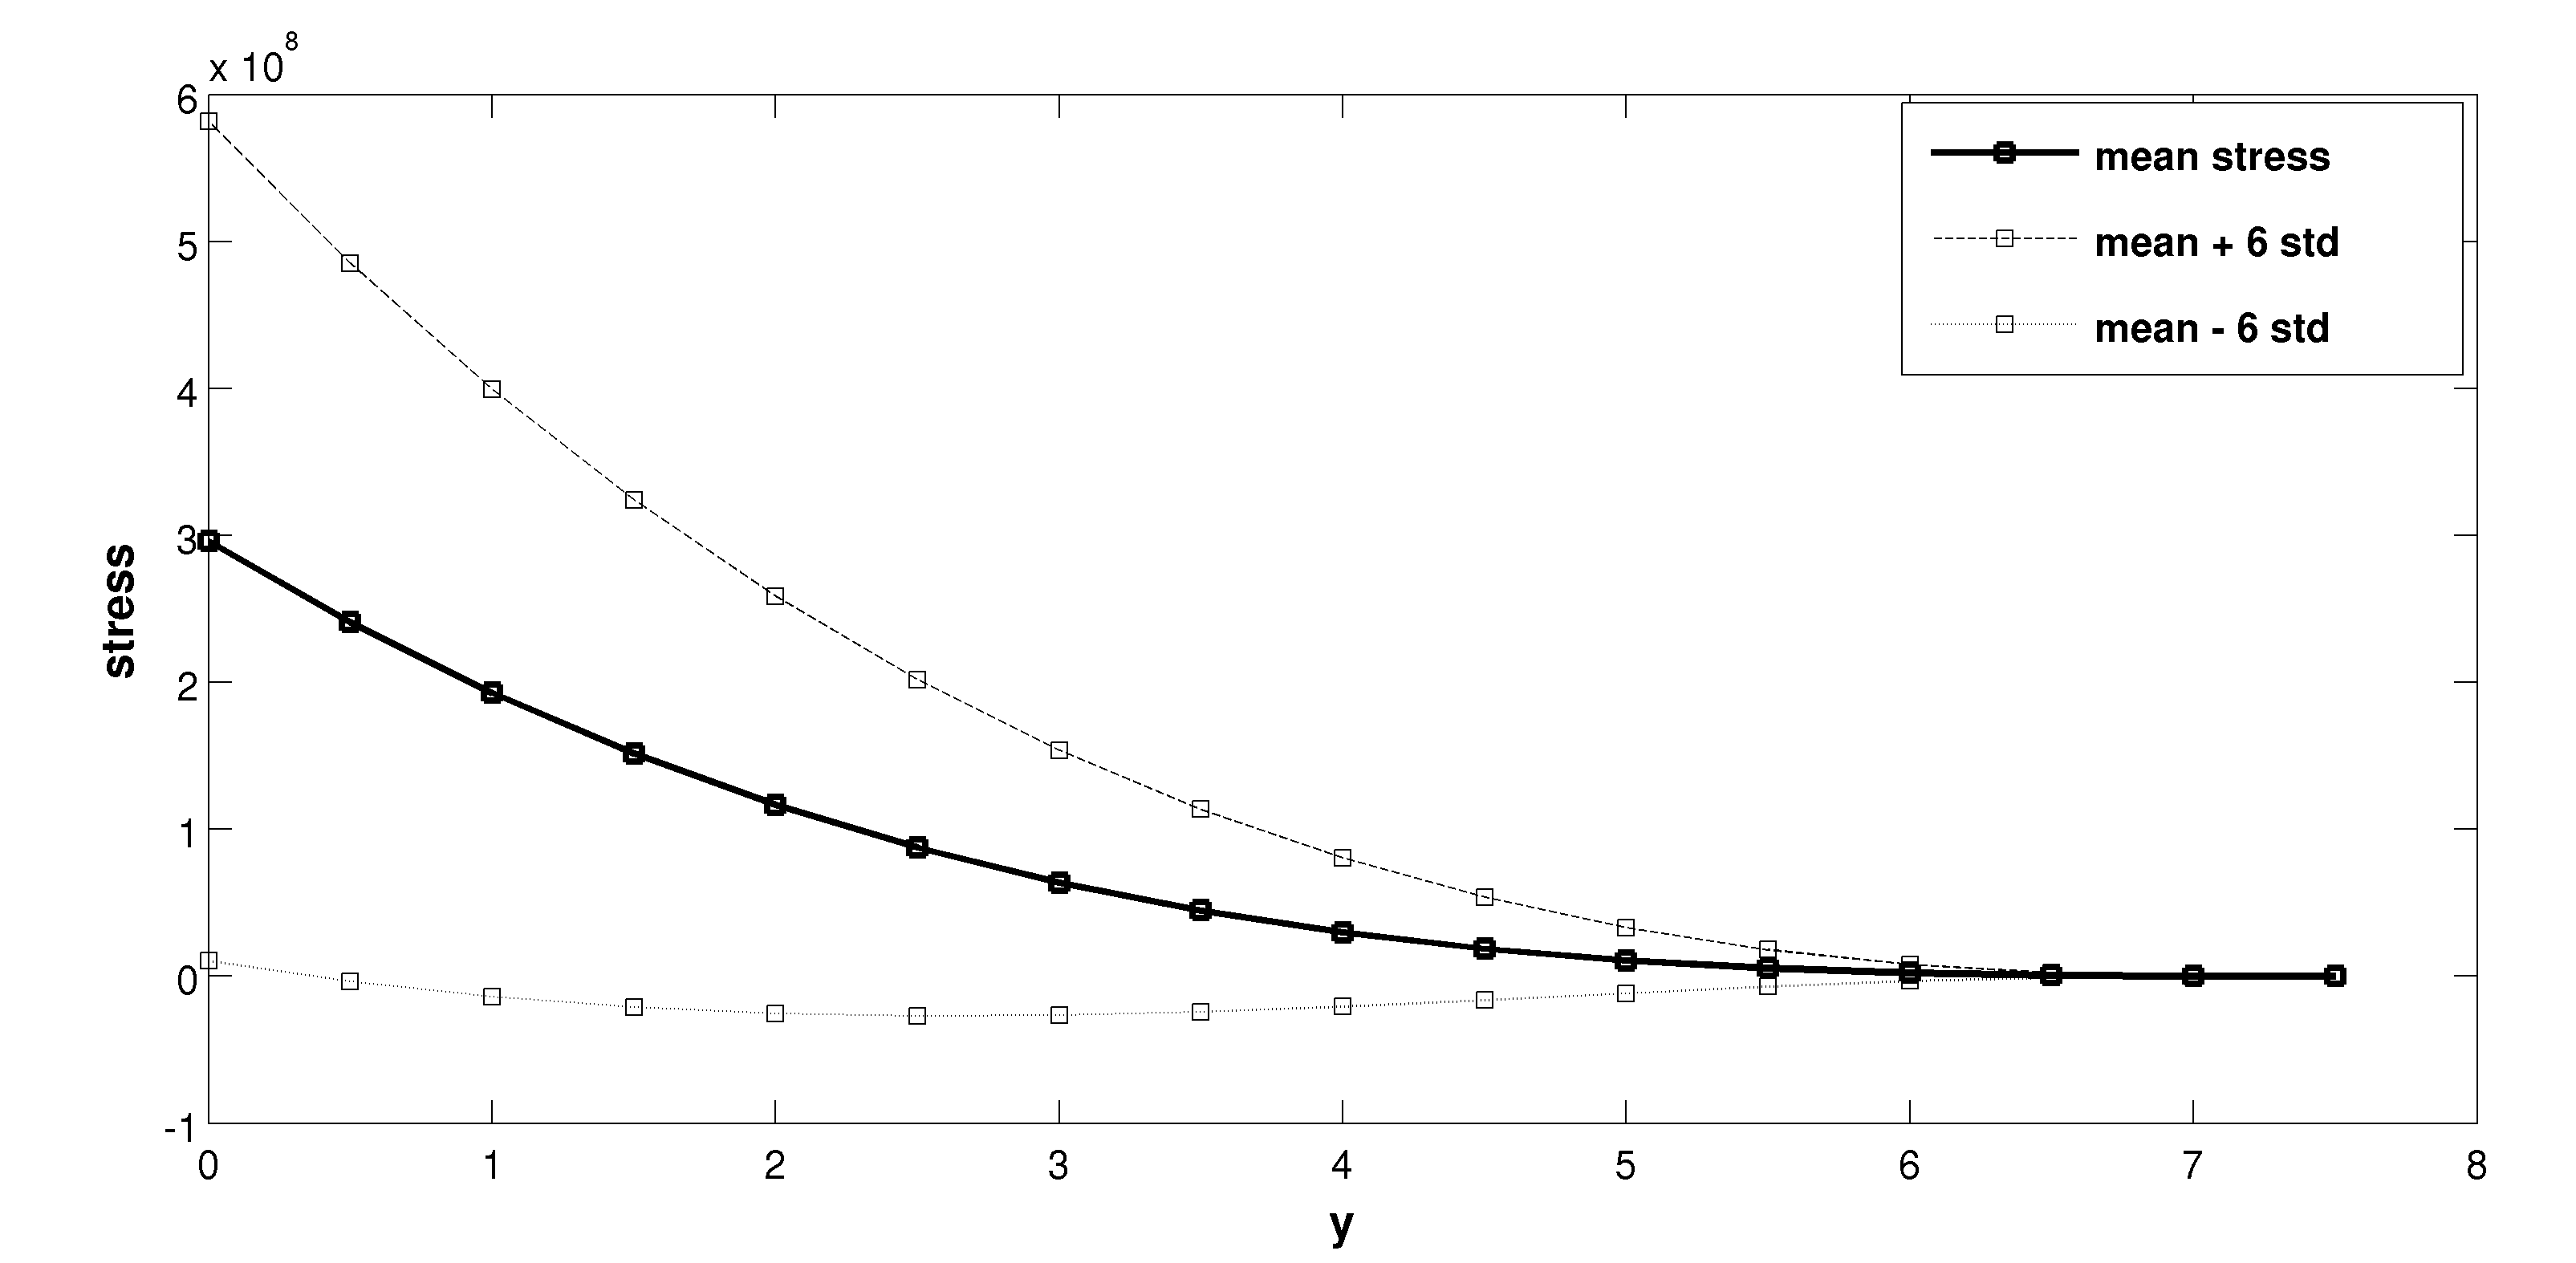
\includegraphics[width=0.7\linewidth]{nomStress}
		\caption{Stress Distribution from Nominal Configuration}
		\label{fig:nomstress}
	\end{figure}
\begin{figure}[H]
	\centering
	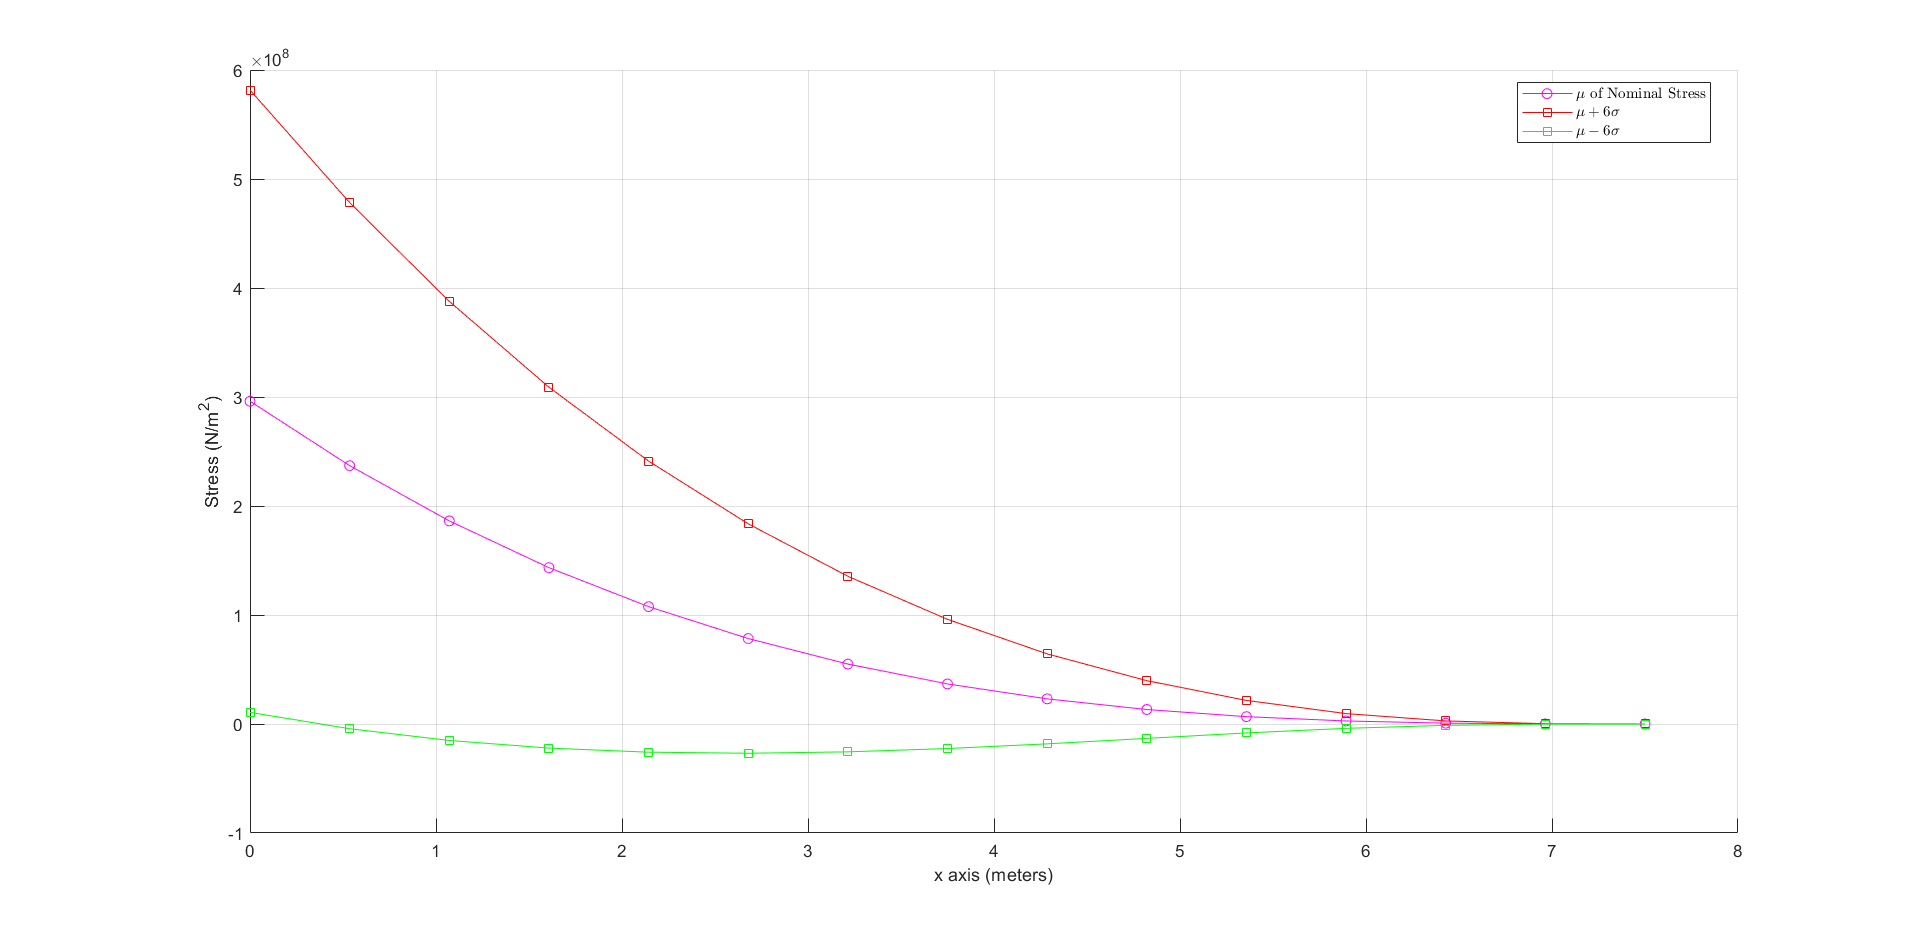
\includegraphics[width=0.7\linewidth]{codeNomMass}
	\caption{Stress Distribution from Nominal Configuration From Code}
	\label{fig:codenommass}
\end{figure}

	The MATAB code outputs the stress associated with the nominal configuration seen in figure \ref{fig:codenommass}. These plots are nearly identical, which means the code is working as we expect it to. 
	
	Running the MATLAB code at 15 elements and 3 collection points gave a result of 8.56387 kg, a little more than 70\% less than nominal. The output from MATLAB's fmincon may be seen in figure \ref{fig:fminconoutput} and the resulting stress and geometry may be seen in figure \ref{fig:coderesultsall}. 
	
	\begin{figure}[H]
		\centering
		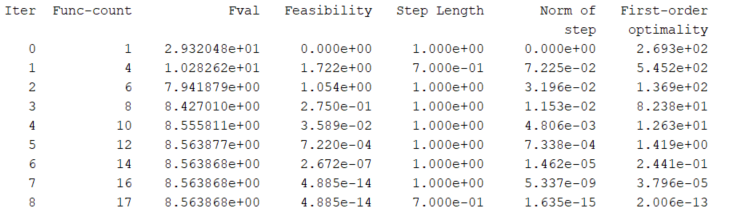
\includegraphics[width=0.7\linewidth]{FminConOutPut}
		\caption{Output from fmincon}
		\label{fig:fminconoutput}
	\end{figure}
	
	
	\begin{figure}[H]
		\centering
		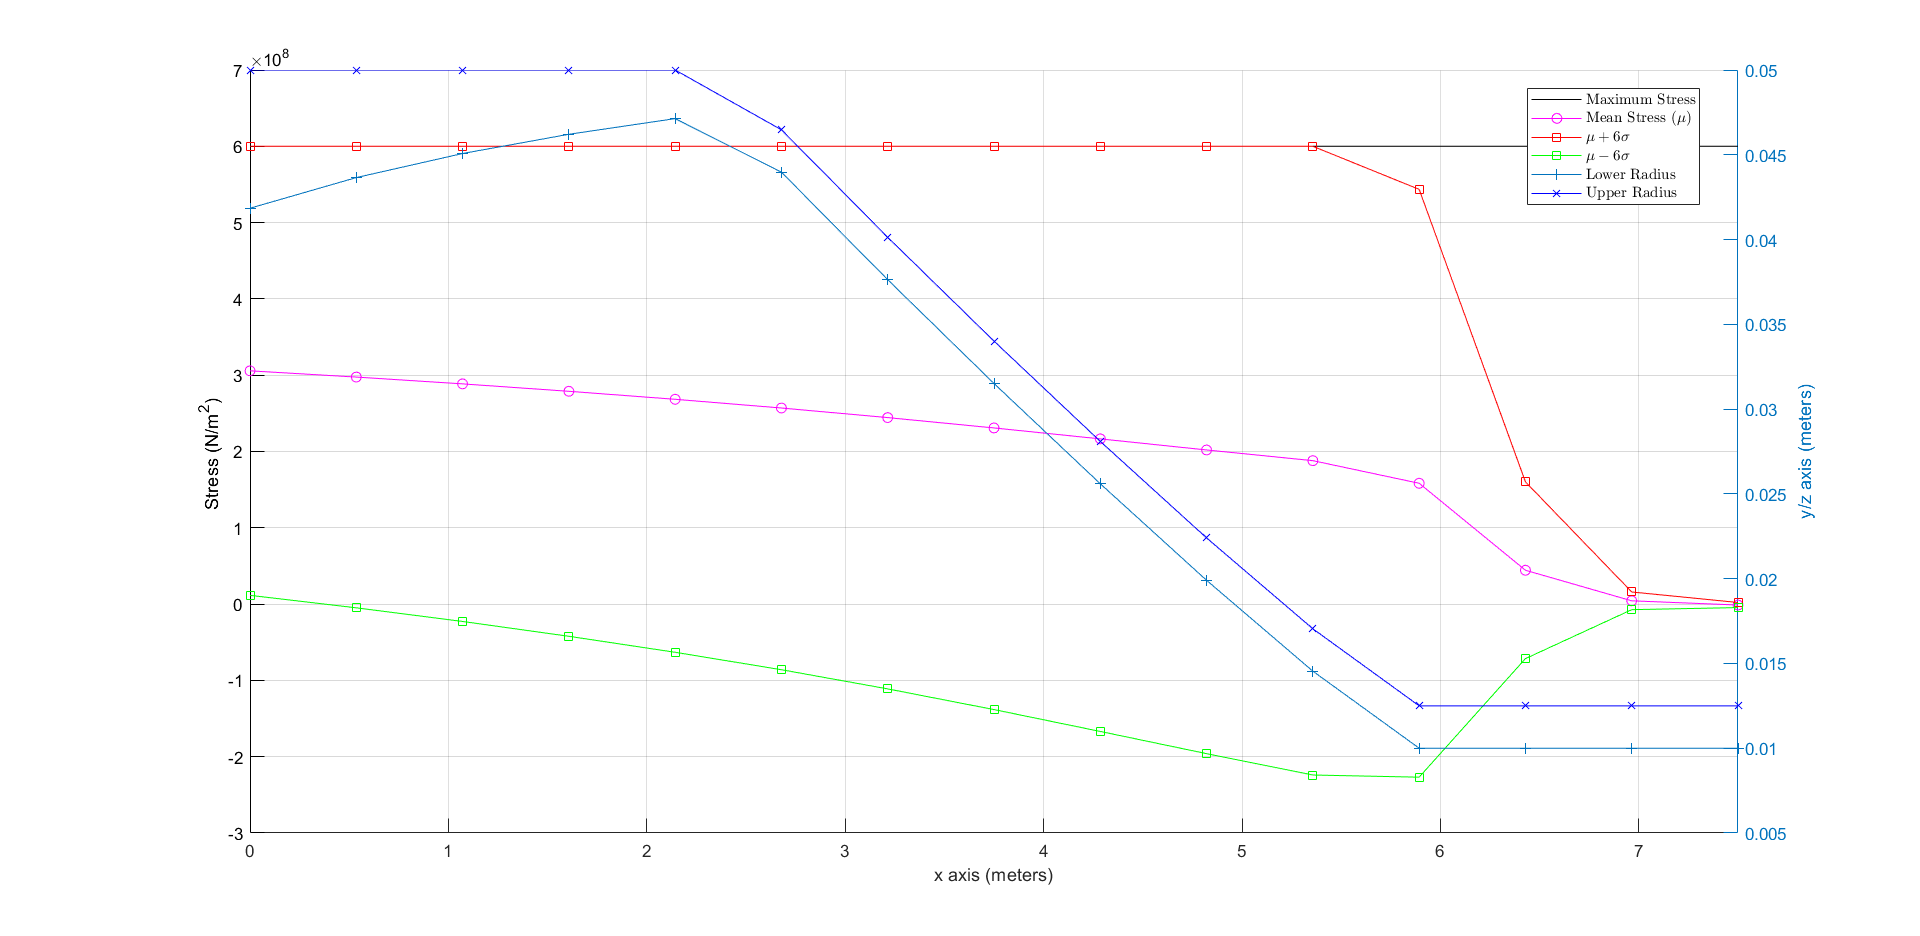
\includegraphics[width=0.7\linewidth]{codeResultsAll}
		\caption{Spar Stress and Geometry  at 15 elements, and 3 collection points. }
		\label{fig:coderesultsall}
	\end{figure}
	
	

	
	Comparing this with the results from project 2 (optimal mass of 4.343), seen in figure \ref{fig:geovstress} shows the spars have a similar shape. Both spars start at a maximum $I_{yy}$ at the root to handle the stress (as the highest force is applied at the root). From there it decreases the mass by first shrinking the thickness, until the minimum thickness is hit. Then it decreases the mass by shrinking the inner radius while keeping the spar able to handle the stress. Eventually it hits a point where the radius and the thickness cannot be shrunk, and this the spar stays at this minimum cross section. However the spar from project 2 does not have to deal with six standard deviations of uncertainty, and can minimize it's mass far more.
	
	\begin{figure}[H]
		\centering
		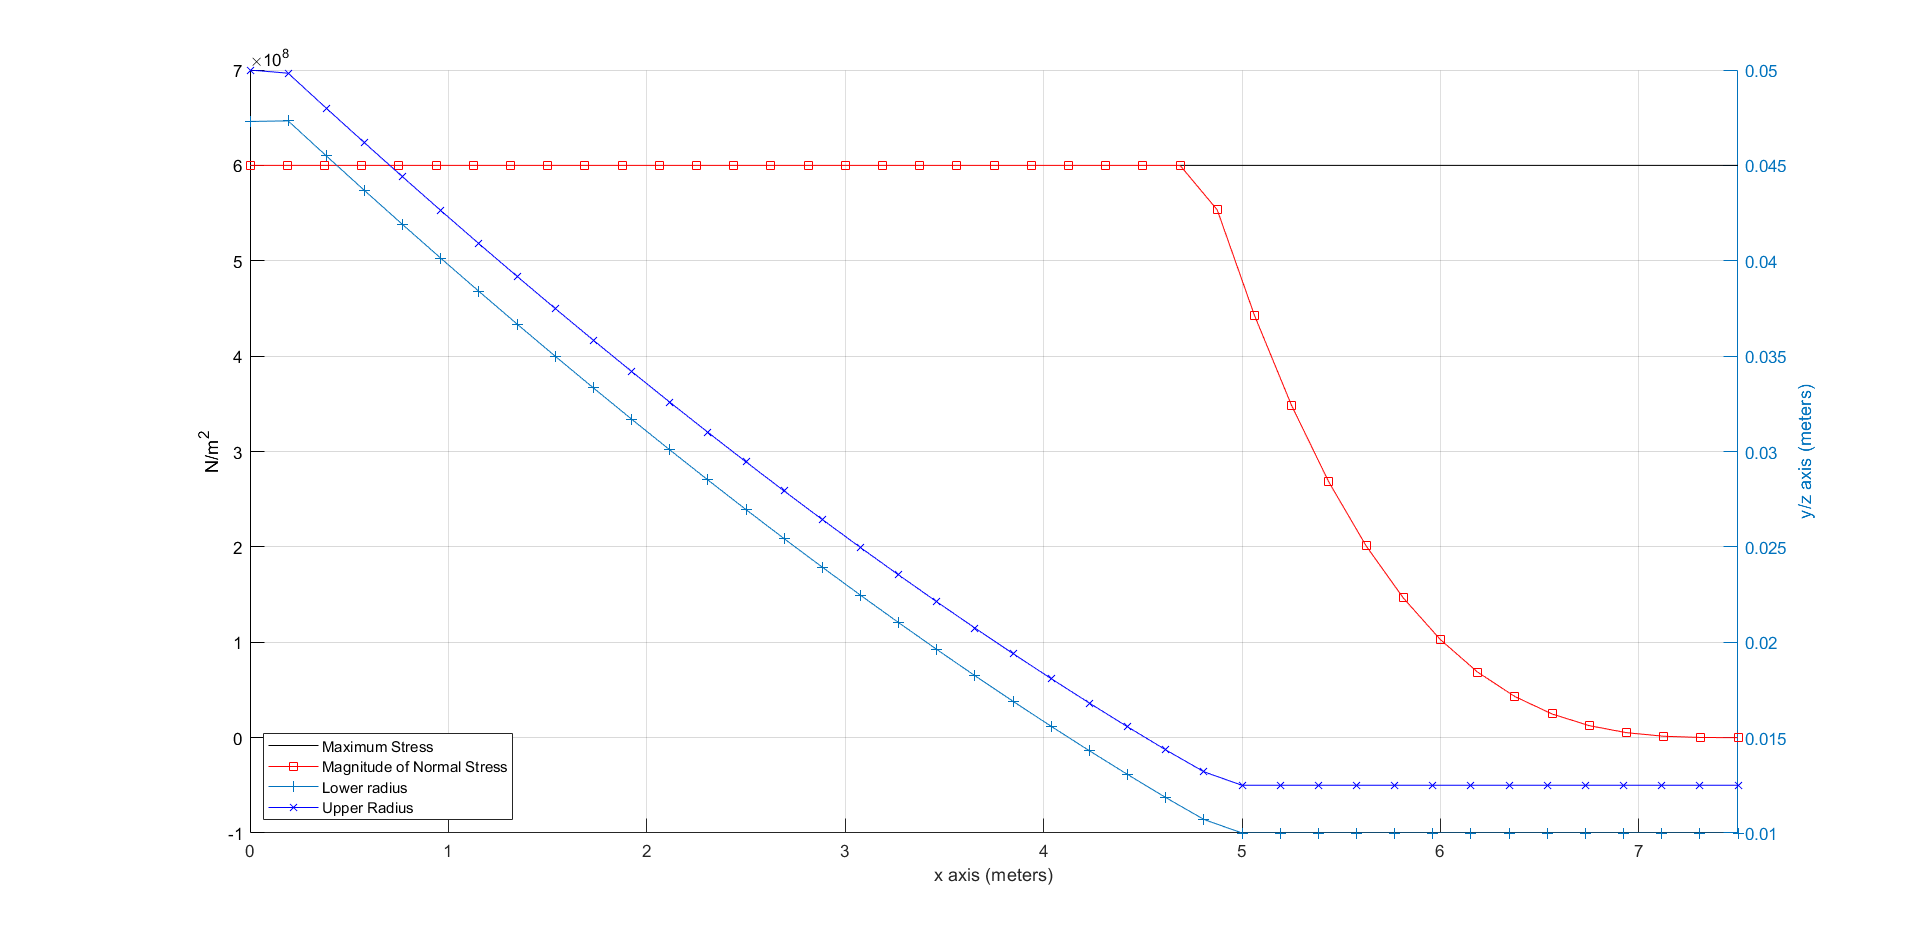
\includegraphics[width=0.7\linewidth]{geoVstress}
		\caption{Geometry of spar and stress of spar from project 2.}
		\label{fig:geovstress}
	\end{figure}
	
	
	What will happen if the code is run for more that three collection points? Running the code at six collection points provided a spar with a mass of 8.56387 kg and a geometry and stress seen in figure \ref{fig:fivecolcresults}.
	
	
	\begin{figure}[H]
		\centering
		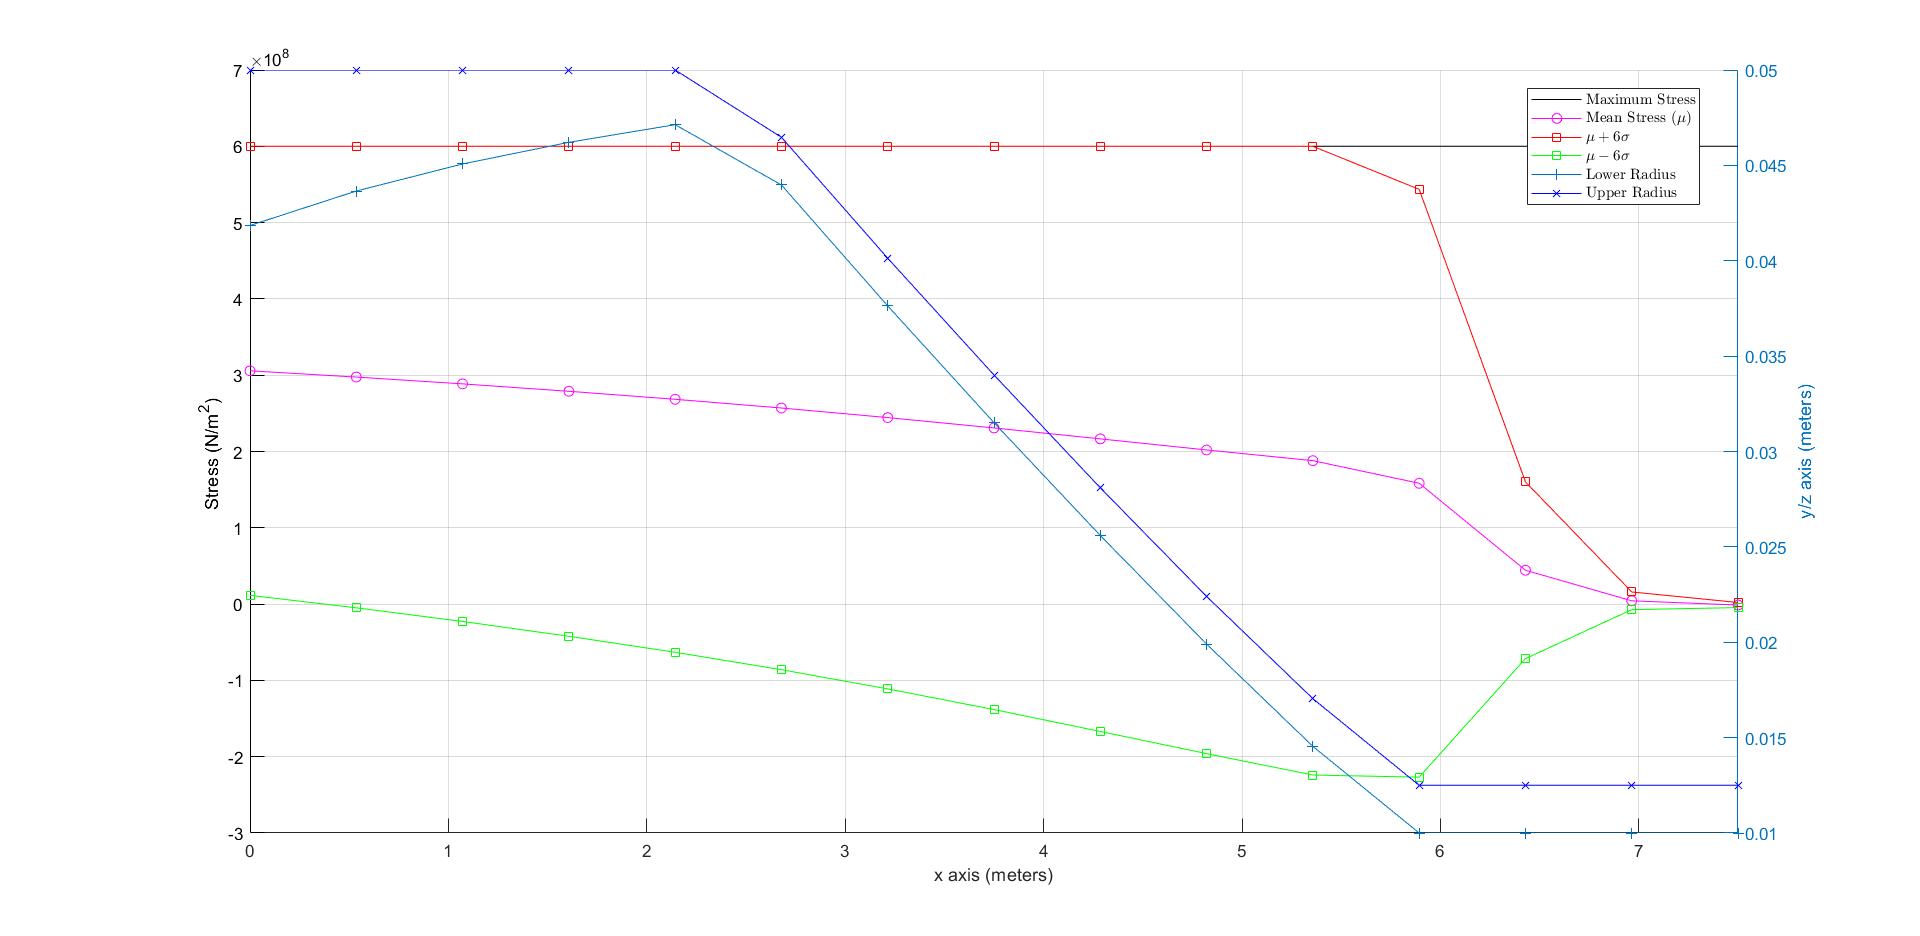
\includegraphics[width=0.7\linewidth]{fiveColcResults}
		\caption{Spar Stress and Geometry  at 15 elements, and 5 collection points.}
		\label{fig:fivecolcresults}
	\end{figure}

	This the results at five collection points are no different than the results at three collection points. In fact if the code is run for different numbers of elements and collection points(as seen in figure \ref{fig:massallplt}) the mass never changes due to the number of collection points, it only changes due to the number of elements.
	
	\begin{figure}[H]
		\centering
		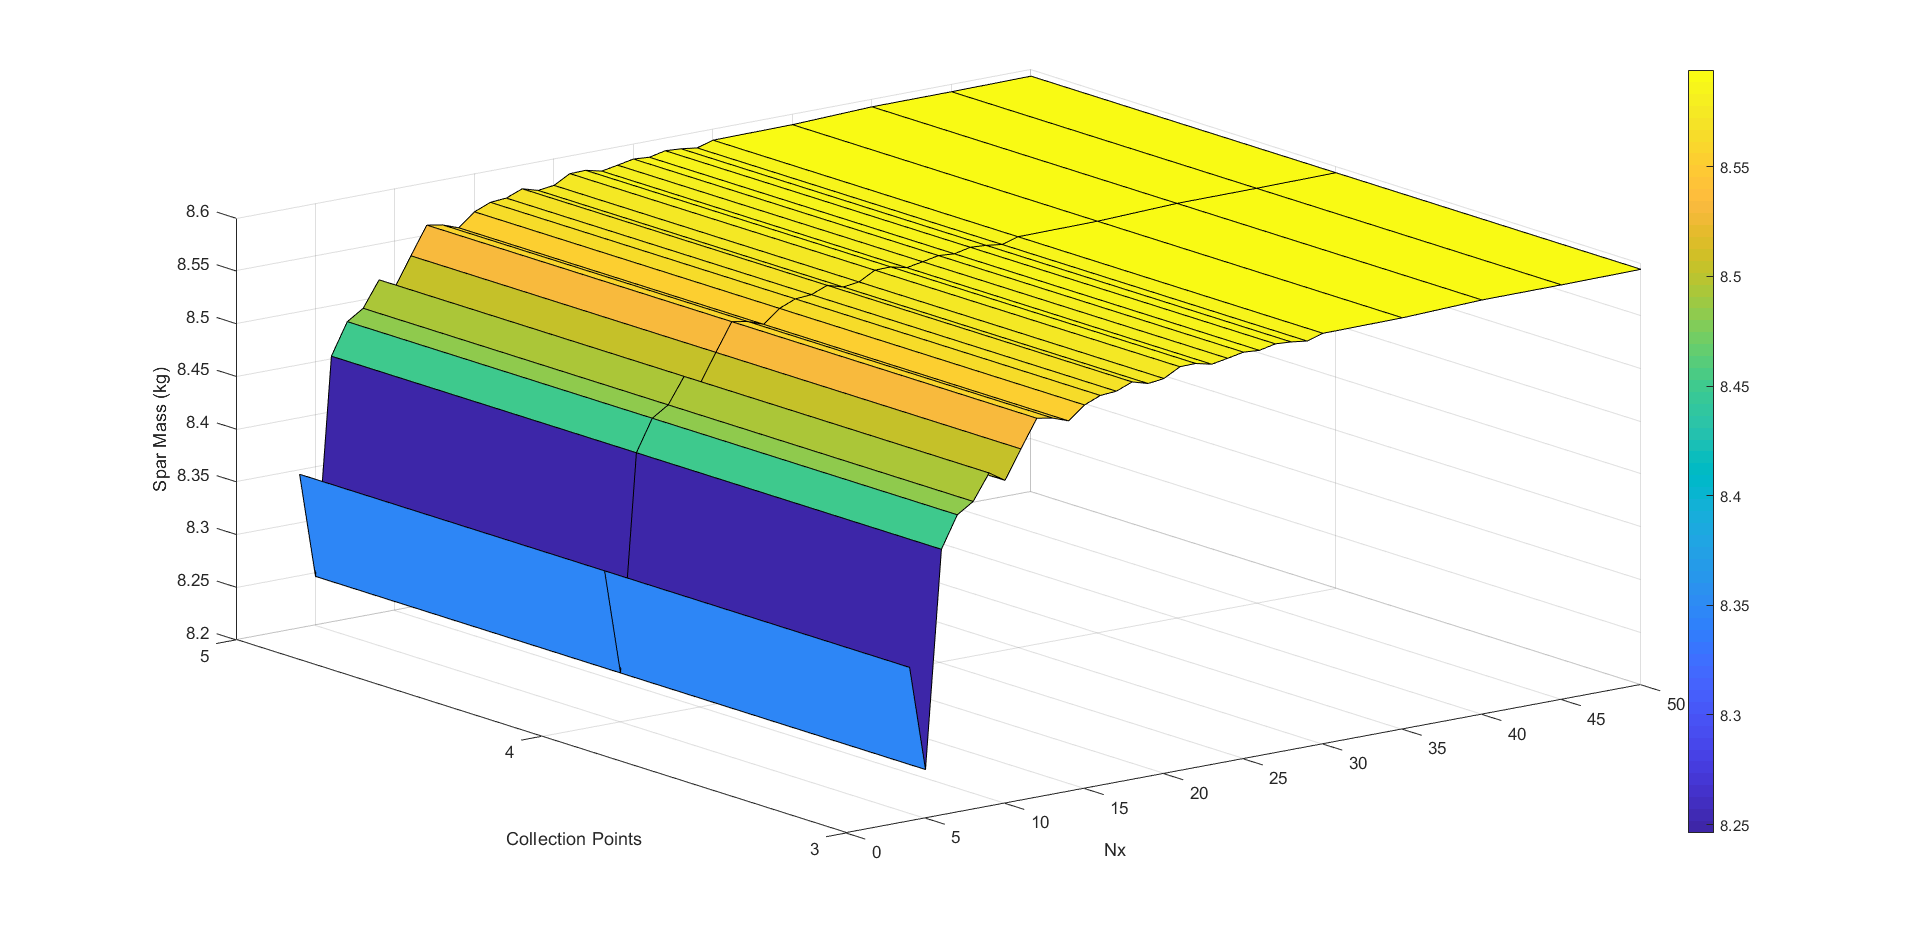
\includegraphics[width=0.7\linewidth]{massAllPlt}
		\caption{Mass vs number of collection points and number of elements}
		\label{fig:massallplt}
	\end{figure}

	As a final check on convergence, we plot the displacement of the tip of the spar vs the number of nodes. This relation, seen in figure \ref{fig:tipdisplacment} shows that the displacement of the tip of the spar changes rapidly with the number of elements at first, but soon settles to a value of 0.681 meters. It stays there even though the number of elements increases.
	
	\begin{figure}
		\centering
		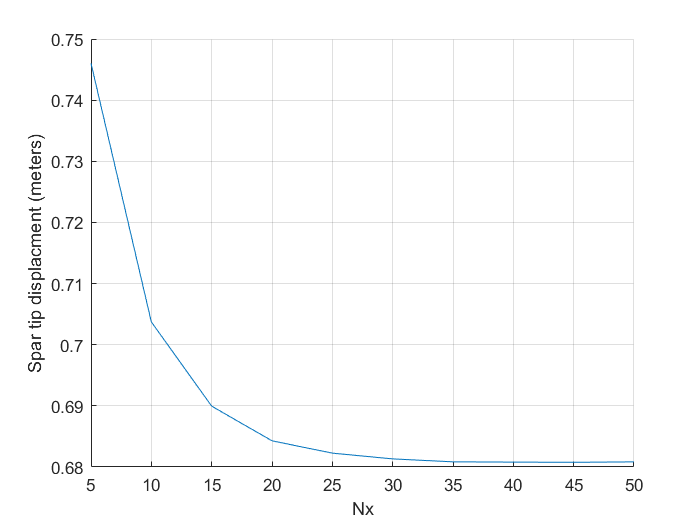
\includegraphics[width=0.7\linewidth]{tipDisplacment}
		\caption{Spar Tip displacement}
		\label{fig:tipdisplacment}
	\end{figure}
	
	
	
	


	

	
	\section{Conclusions}
	%It is a common falicy that alimuinum is used in aeroplanes because it is lighter than steel. 
	
	The MATLAB results are what would be expected. When dealing with a large uncertainty, the spar will be heavier than the spar that was developed in uncertainty free project 2. The spar has a similar geometry to project 2's spar, just scaled to handle the uncertainty. The $I_{yy}$ must be at it's maximum near the root, then as it moves down the wing it can shrink to decrease mass. It first shrinks the thickness, and when it hits the minimum thickness it shrinks the radius. However at a certain point the radius can shrink no more and it stays at the minimum radius and thickness for the rest of the spar length. Like project 2, the stress is kept at the appropriate factor of safety for as long as possible.\par 
	
	What was unexpected was that the number of collection points had no difference in the resulting mass. The only thing that changed the mass was the number of elements the spar was made up of. 
	
	Something that engineers must take into account when designing models is the run time cost. The time to run each calculation at a different number of nodes and collection points is seen in figure \ref{fig:comptime}.\par 
	%\newpage
	\begin{figure}[H]
		\centering
		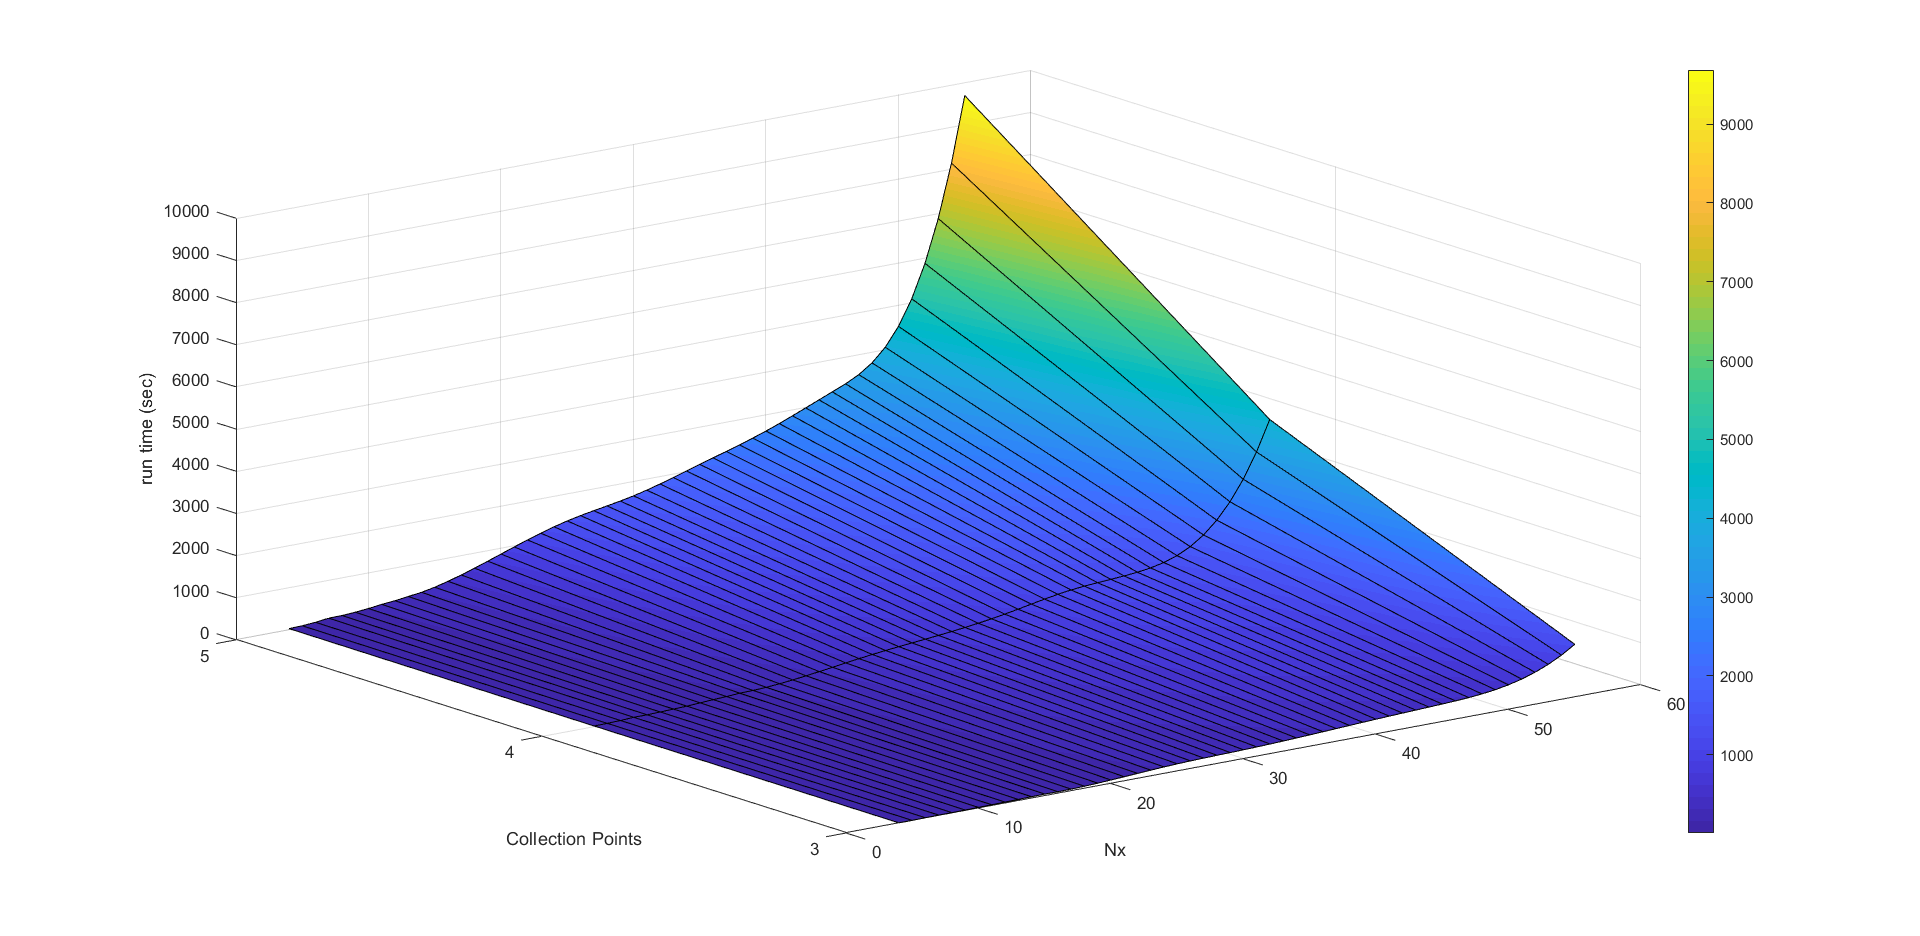
\includegraphics[width=0.7\linewidth]{runTimePlt}
		\caption{Time to run optimization vs the number of collection points and nodes}
		\label{fig:comptime}
	\end{figure}
	
	 As the number of nodes and collection points increases, so too does the time to run the model increase. This is important as some models may take to long to run for their results to be useful. Additionally it can be seen that once the number of nodes reaches a certain number, the mass changes very little with subsequent increases. In figure \ref{fig:massallplt}, this point is around 40 nodes. Thus the return of accuracy over run time is so small that it is not worth running the code past this point.\par 

	
	
		
	\section{References}
	\label{sec:References}
		\bibliographystyle{ieeetran}
	\bibliography{ref}%.bib}
	\noindent This report was written by ID: 6110 in Latex. If desired the source code may be provided.\par 
	%\bibliographystyle{plain}
	%\newpage
	\section{Appendix: MATLAB Code}
	\lstset{language=Matlab,%
		%basicstyle=\color{red},
		breaklines=true,%
		morekeywords={matlab2tikz},
		keywordstyle=\color{blue},%
		morekeywords=[2]{1}, keywordstyle=[2]{\color{black}},
		identifierstyle=\color{black},%
		stringstyle=\color{mylilas},
		commentstyle=\color{mygreen},%
		showstringspaces=false,%without this there will be a symbol in the places where there is a space
		numbers=left,%
		numberstyle={\tiny \color{black}},% size of the numbers
		numbersep=9pt, % this defines how far the numbers are from the text
		emph=[1]{for,end,break},emphstyle=[1]\color{red}, %some words to emphasise
		%emph=[2]{word1,word2}, emphstyle=[2]{style},    
	}
	%\subsection{Master Script}
	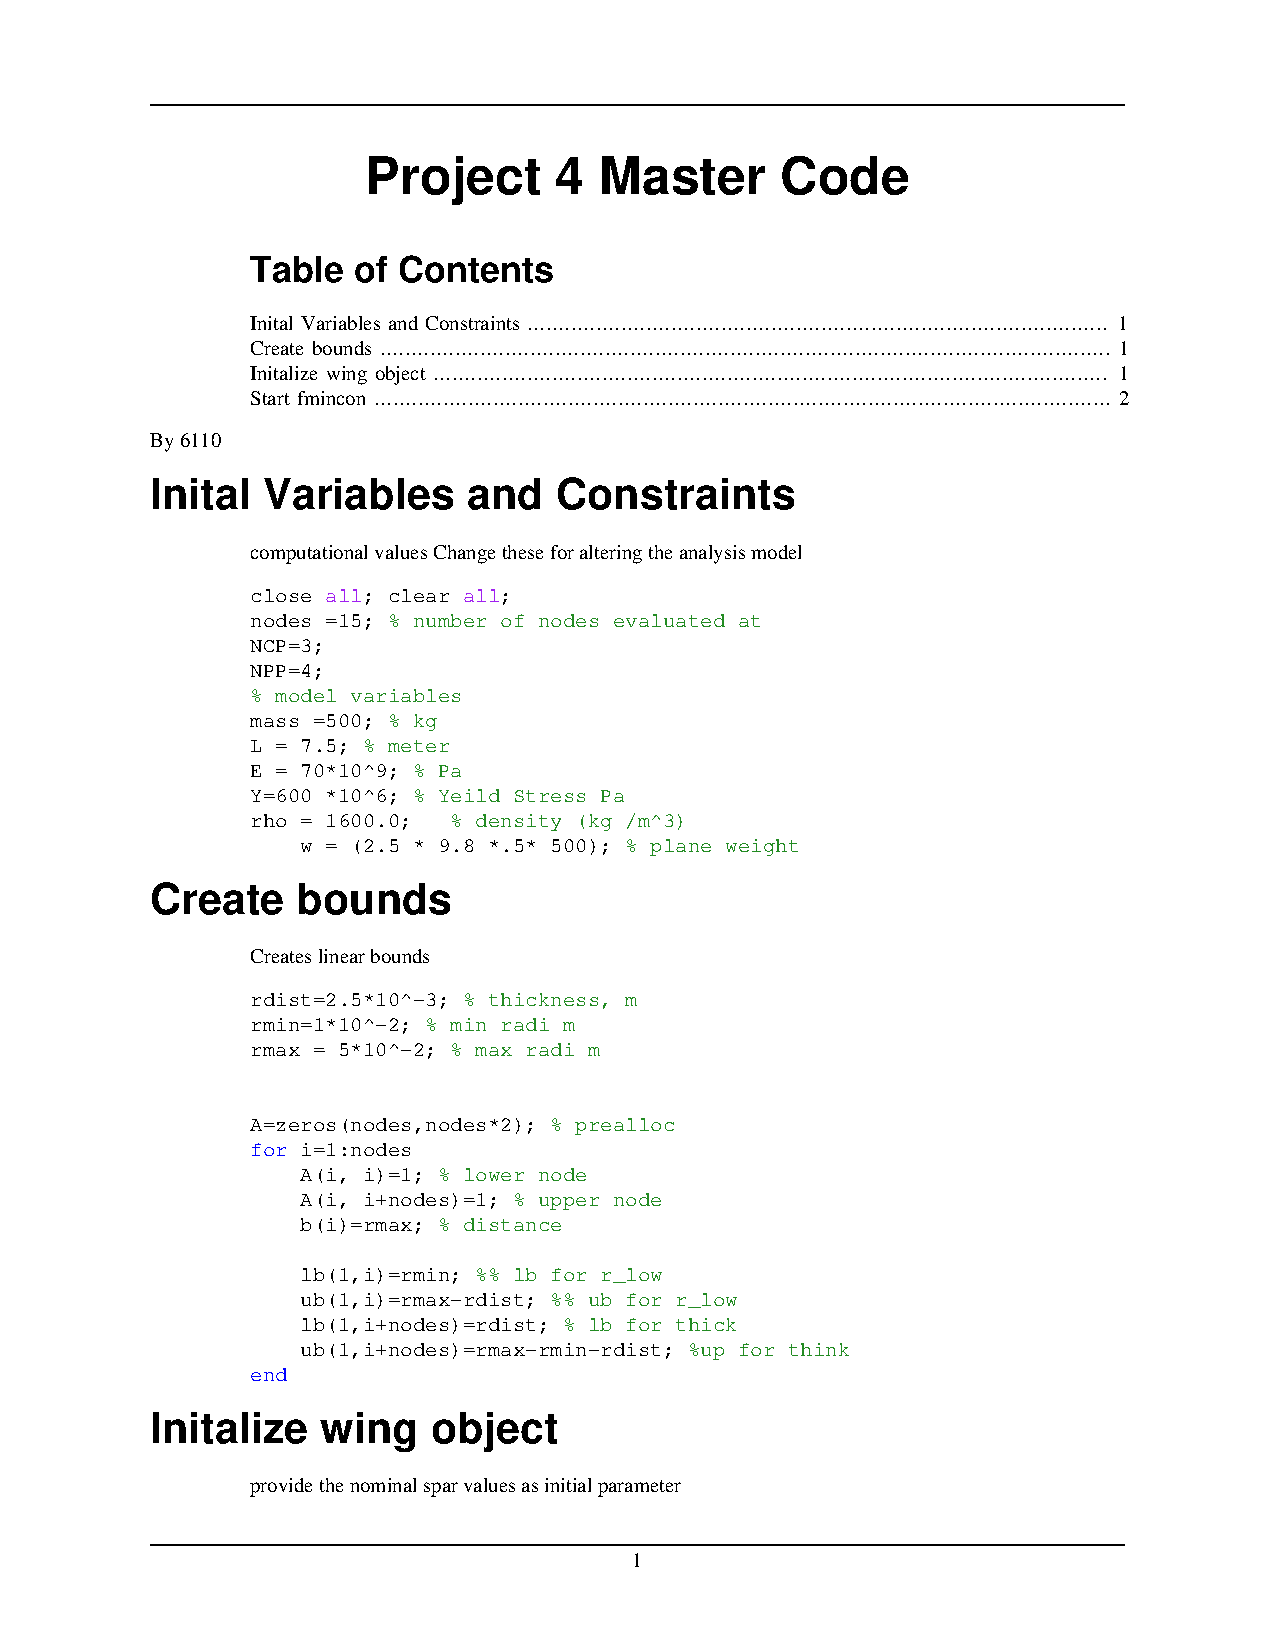
\includepdf[pages=-]{C:/Users/Philip/Documents/GitHub/DesignOpt/Project4/html/Project_4_master.pdf}

	%\newpage
	%\subsection{Spar Class}
	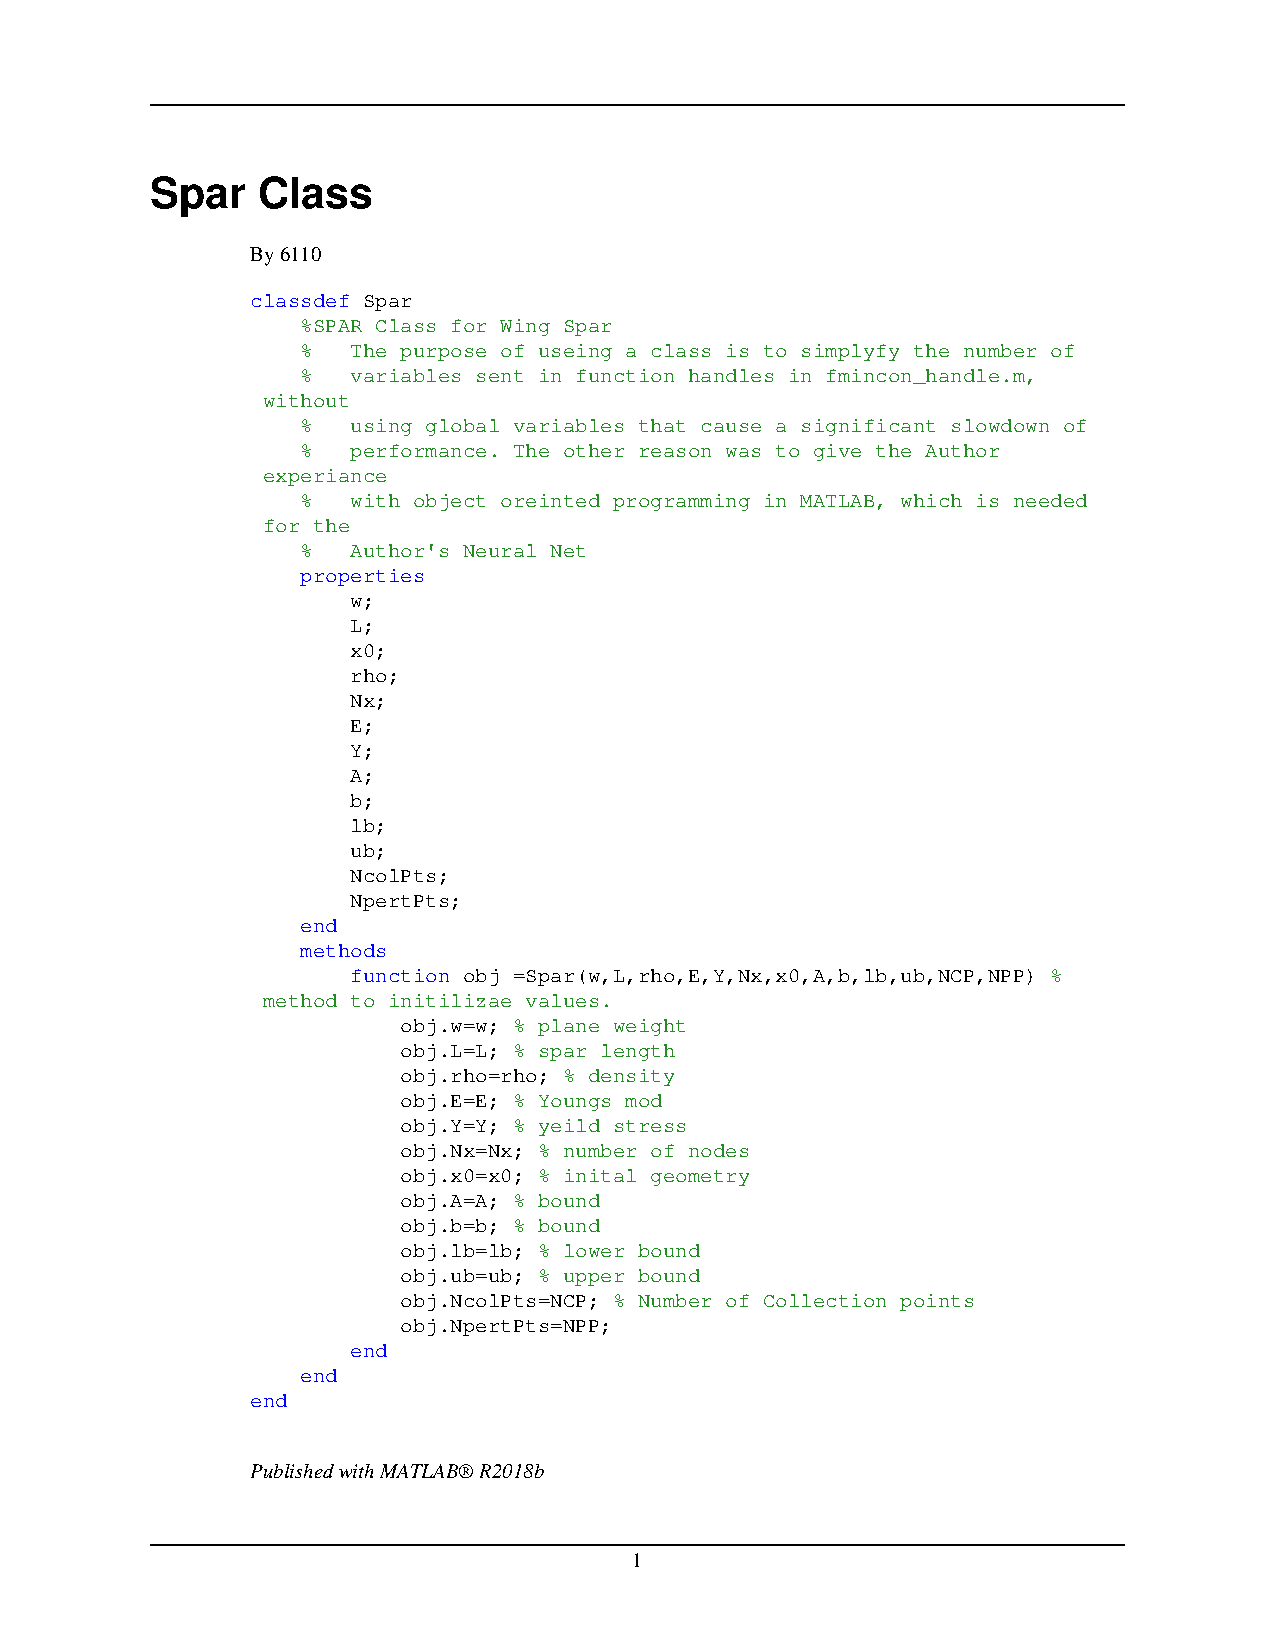
\includepdf[pages=-]{C:/Users/Philip/Documents/GitHub/DesignOpt/Project4/html/Spar.pdf}
	%\lstinputlisting{project_2_master.m}
	%\newpage
	
	%\subsection{fmincon\_handle.m}
	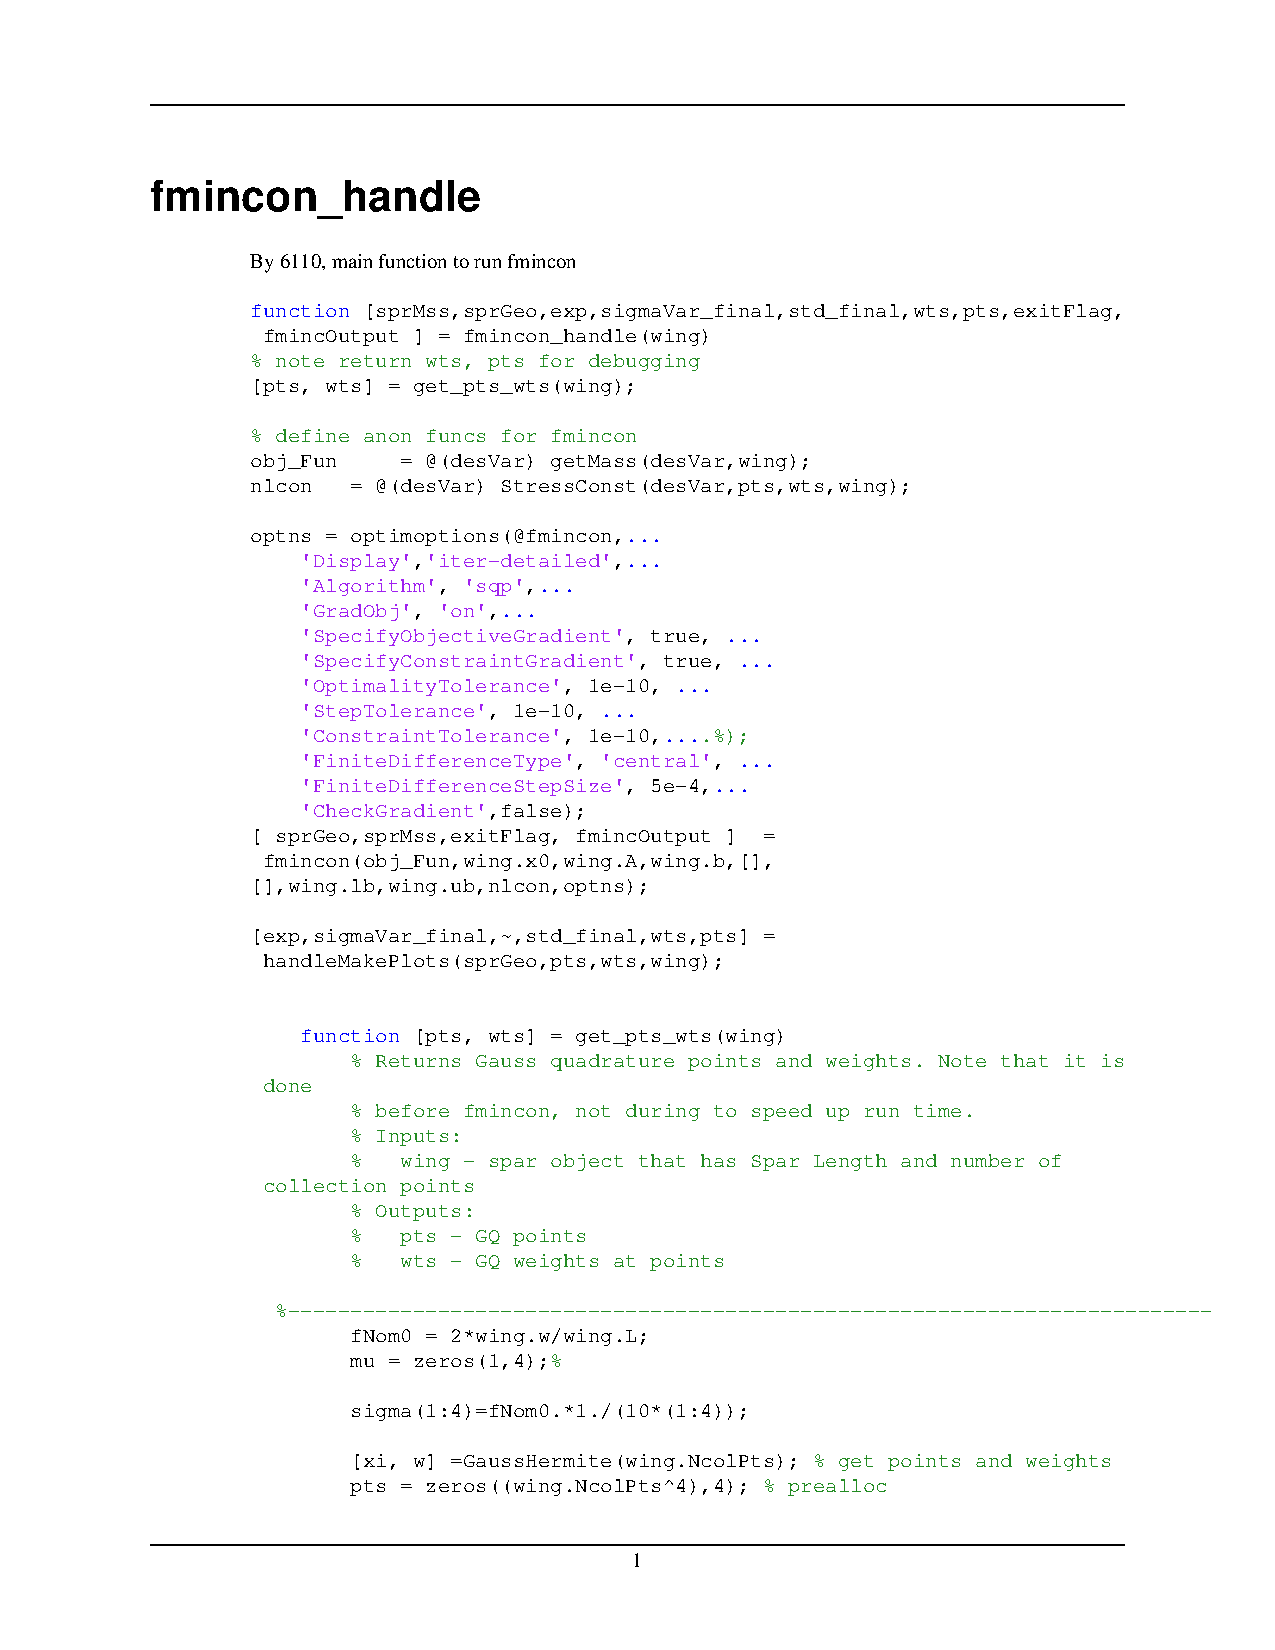
\includepdf[pages=-]{C:/Users/Philip/Documents/GitHub/DesignOpt/Project4/html/fmincon_handle.pdf}
	%\lstinputlisting{project_2_master.m}
	%\newpage
	
	%\subsection{Make Plots}
	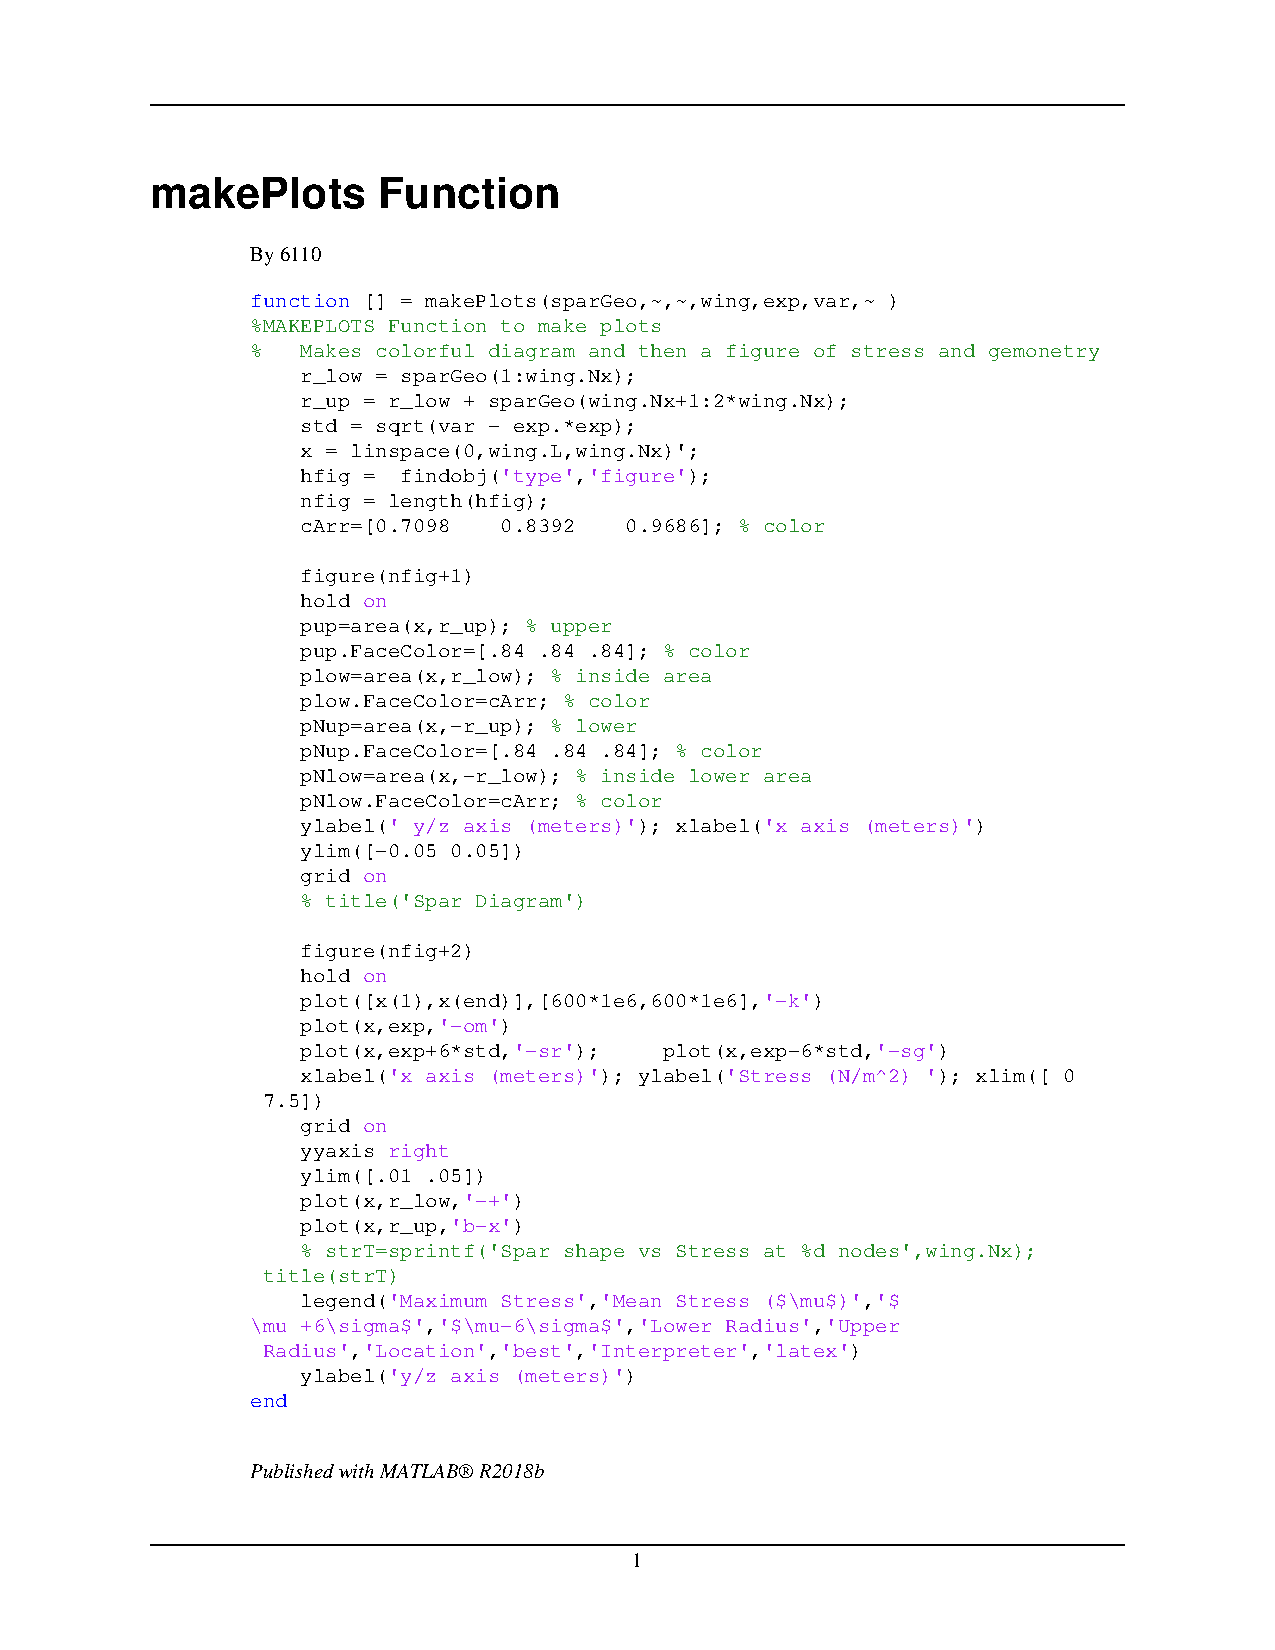
\includepdf[pages=-]{C:/Users/Philip/Documents/MATLAB/Fall2018/DesignOpt/Project_4/Final_Version/html/makePlots.pdf}
	
	\iffalse
	\lstinputlisting{project_2_master.m}

	\subsection{runFmincon.m}
	\lstinputlisting{runFmincon.m}
	%\newpage
	\subsection{stressCon.m}
	\lstinputlisting{stressCon.m}
	\newpage
	\subsection{cStep.m}
	\lstinputlisting{cStep.m}
	
	\subsection{cStep\_nonlinCon.m}
	\lstinputlisting{cStep_nonlinCon.m}
	
	\subsection{Iyy\_zmax\_from\_rLU.m}
	\lstinputlisting{Iyy_zmax_from_rLU.m}

	\subsection{create\_x\_from\_nodes\_Best.m}
	\lstinputlisting{create_x_from_nodes_Best.m}
	\subsection{create\_x\_from\_nodes.m}
	\lstinputlisting{create_x_from_nodes.m}
	\subsection{create\_r\_from\_x.m}
	\lstinputlisting{create_r_from_x.m}
	\subsection{create\_constraints.m}
	\lstinputlisting{create_constraints.m}
	\subsection{makePlots.m}
	\lstinputlisting{makePlots.m}
	\fi
	
	


%    \bibliography{ref}%.bib}
%\bibliographystyle{plain}



	
	
	% --------------------------------------------------------------
	%     You don't have to mess with anything below this line.
	% --------------------------------------------------------------
	
\end{document}
